\documentclass[paperwidth=40in,paperheight=32in,landscape]{baposter} % Set poster size and orientation

\usepackage{amsmath,amssymb}
\usepackage{graphics}
\graphicspath{{images/}}
\usepackage{color}
\usepackage{multicol}
	\setlength{\columnseprule}{1pt}
	\def\columnseprulecolor{\color{black}}
	
\newcommand{\headshotsize}{0.95in}
% \newcommand{\headshotsize}{1.0in}
%%% Color Definitions %%%

\definecolor{cuGold}{cmyk}{0, .10, .48, .22}
\definecolor{cuBlack}{cmyk}{0, 0, 0, 1.00}
\definecolor{cuDarkGray}{cmyk}{.38, .28, .21, .63}
\definecolor{cuLightGray}{cmyk}{.16, .11, .11, .29}

\definecolor{bordercol}{RGB}{0,0,0} % Content cell border color
\definecolor{headercol}{RGB}{229,240,241} % Concent cell header fill color
\definecolor{headerfontcol}{RGB}{0,0,0} % Concent cell header text color
\definecolor{boxcol}{RGB}{255,255,255} % Concent cell background color

%%% Document Start %%%

\begin{document}

%%% Poster Settings %%%

\begin{poster}{
	grid = false, % Turns off alignment grid 
	columns = 4, % Sets number of poster columns
	colspacing = 1em,
	headerheight = 0.1\textheight,
	background = plain,
	bgColorOne = cuBlack,
	borderColor = cuGold,
	headerColorOne = cuDarkGray,
	textborder = rounded,
	headerborder = closed,
	headershape = rounded,
	headershade = plain,
	boxshade = plain,
	headerfont = \Large\sf\bf,
	headerFontColor = cuGold,
	boxColorOne = white,
	linewidth = 2pt
}
{

\includegraphics[height=\headshotsize, trim={0.5cm, 1cm, 16.4cm, 0.7cm}, clip=true]{cu_logo}
\hspace{.5cm}
\includegraphics[height=\headshotsize]{NSF_logo.eps}
}
{\sf\bf
	\color{cuGold}
	RBF Quadrature for Neural Fields
}
{
	\color{cuGold}
	Sage B. Shaw$^{1}$, Zack P. Kilpatrick$^1$, and Daniele Avitable$^2$\\
	\small{1: University of Colorado Boulder}
	\small{2: Vrije Universiteit Amsterdam}
}
{

\includegraphics[height=\headshotsize, trim={3cm, 0cm, 3cm, 0cm}, clip=true]{headshot_sage}
\hspace{.5cm}
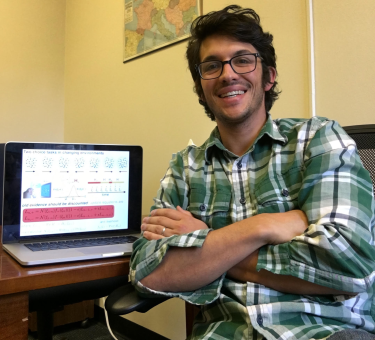
\includegraphics[height=\headshotsize, trim={5.1cm, 6cm, 2cm, 0cm}, clip=true]{headshot_zack}
\hspace{.5cm}
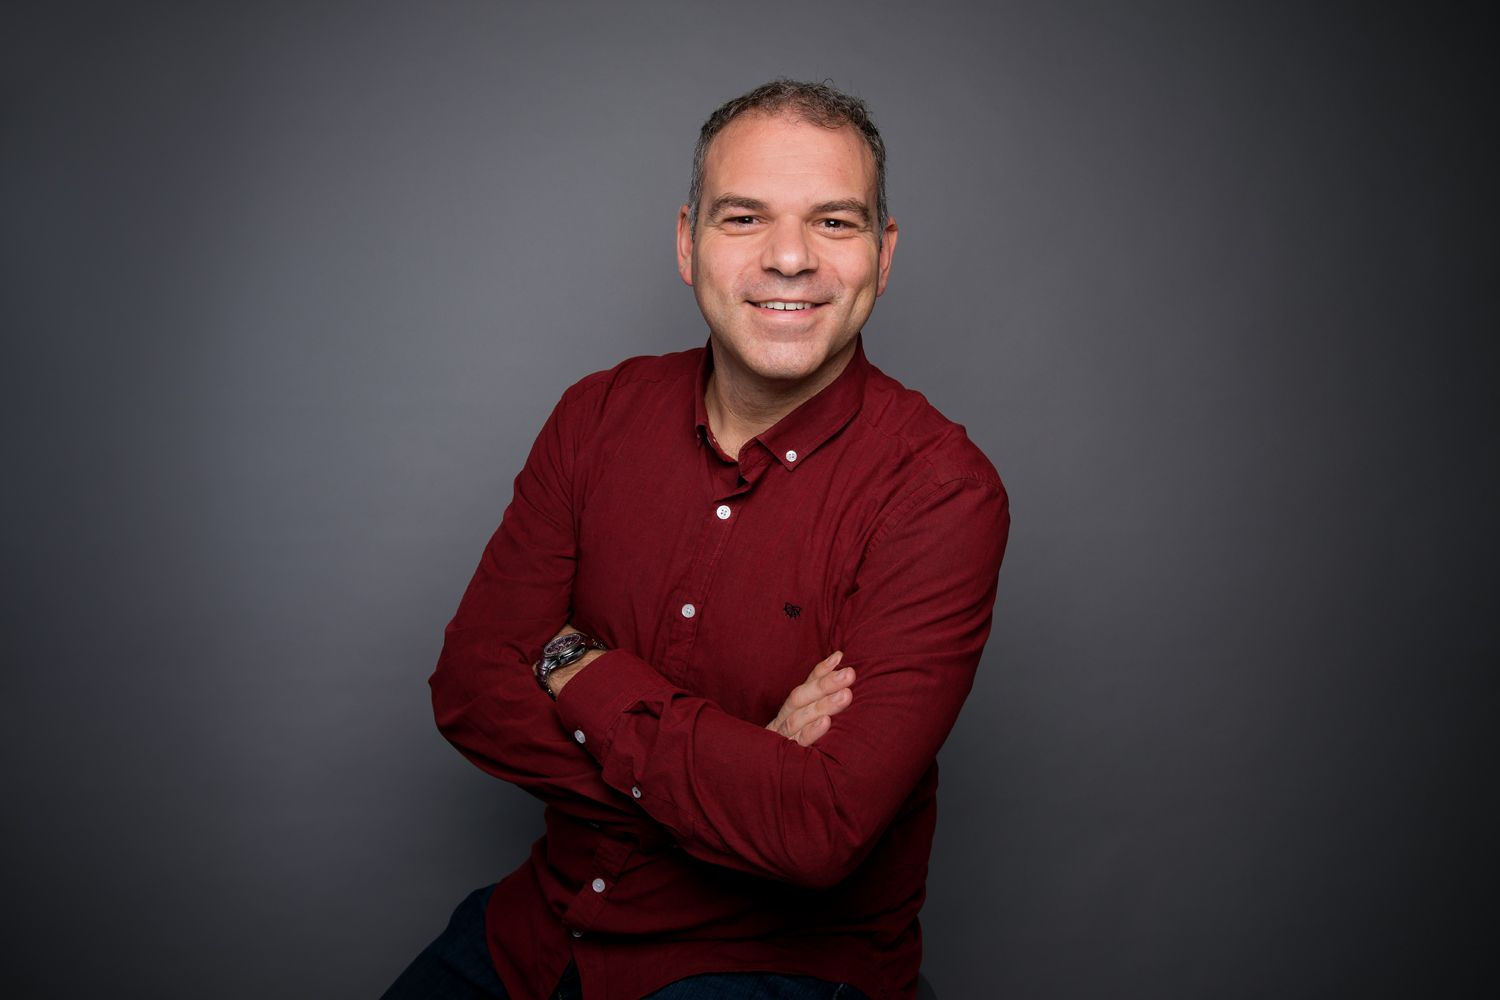
\includegraphics[height=\headshotsize, trim={21cm, 20cm, 18cm, 2cm}, clip=true]{headshot_daniele}
}
%%% Poster Content %%%

%%%%%%%%%%%%%%%%%%%
%%% Column 0
%%%%%%%%%%%%%%%%%%%
\headerbox{Summary}{name = summary, column = 0}{
	% Itemize Example:
	\begin{itemize}
		\setlength\itemsep{0pt}
		\small{
			\item \bf{Scientific Question}
		}
	\end{itemize}
	% Figure Example: 
	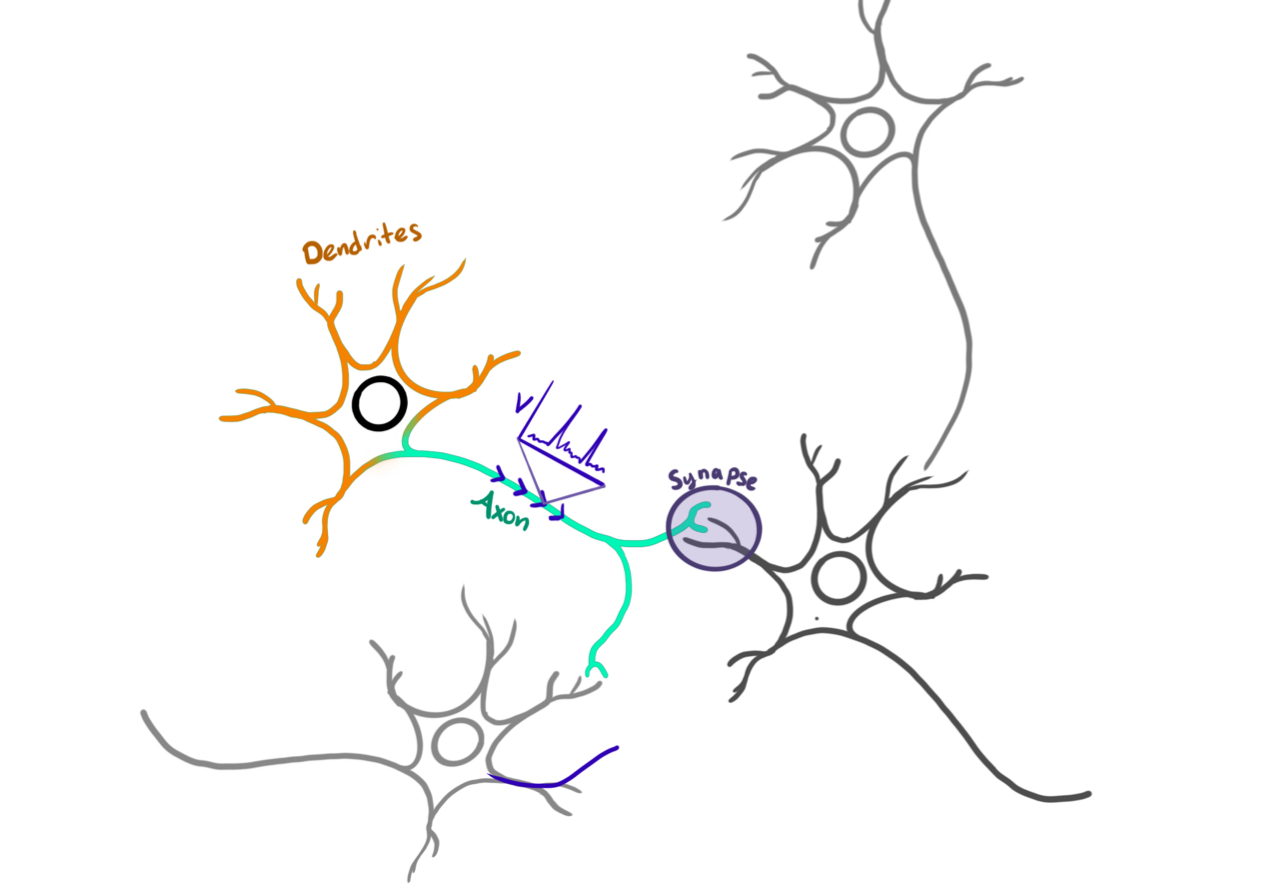
\includegraphics[width=\linewidth]{images/FILENAME}
	% Acknowledgements & References Example:
	\small{This work is supported by GRANT INFORMATION\\
		(1) AUTHORS (YEAR) \textit{JOURNAL}}
}

\headerbox{Neural Field Models}{name = neuralfield, column = 0, below=summary}{
	% Itemize Example:
	\begin{itemize}
		\setlength\itemsep{0pt}
		\small{
			\item \bf{Scientific Question}
		}
	\end{itemize}
	% Figure Example: 
	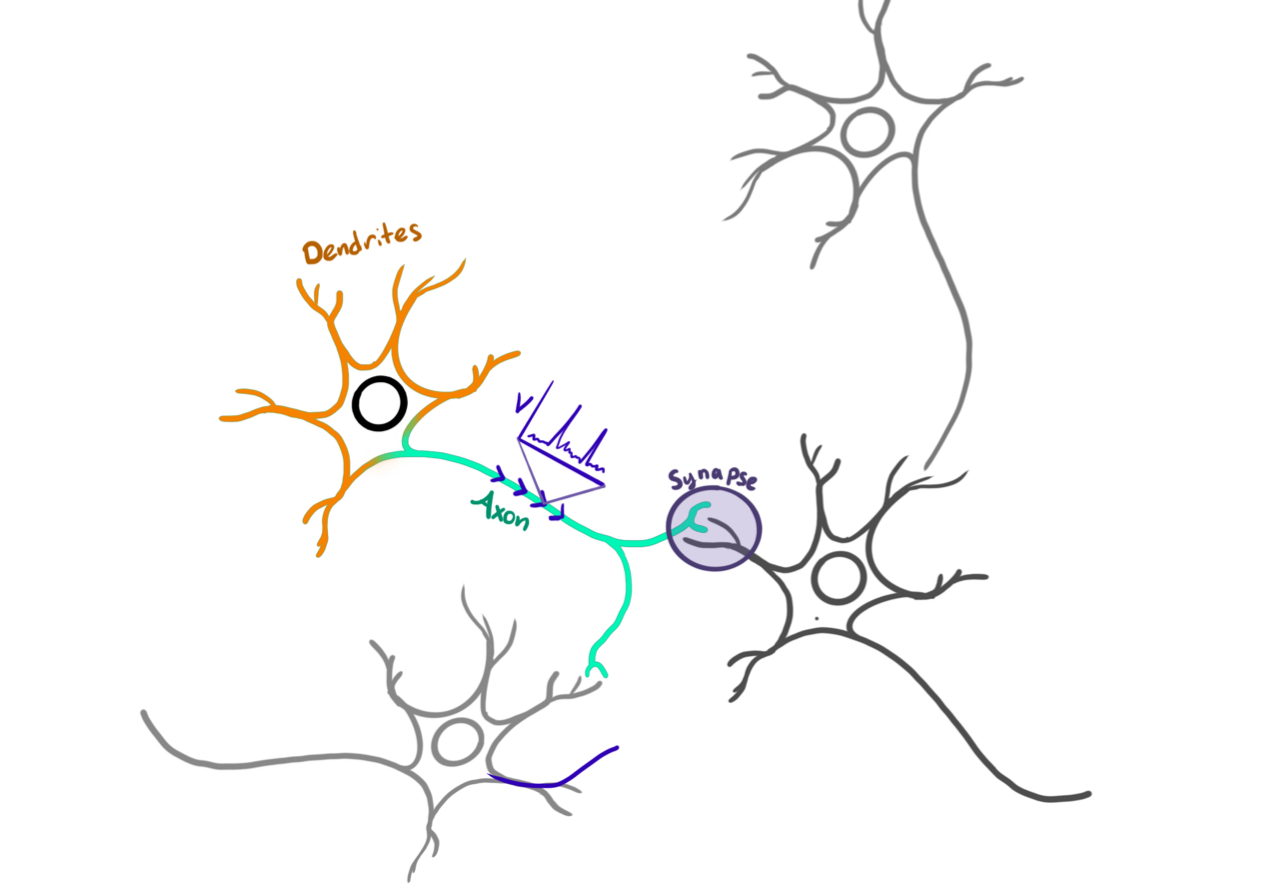
\includegraphics[width=\linewidth]{images/FILENAME}
	% Acknowledgements & References Example:
	\small{This work is supported by GRANT INFORMATION\\
		(1) AUTHORS (YEAR) \textit{JOURNAL}}
}

%%%%%%%%%%%%%%%%%%%
%%% Column 1 
%%%%%%%%%%%%%%%%%%%
\headerbox{RBF-QF}{name = rbfqf, column = 1}{
	% Itemize Example:
	\begin{itemize}
		\setlength\itemsep{0pt}
		\small{
			\item \bf{Scientific Question}
		}
	\end{itemize}
	% Figure Example: 
	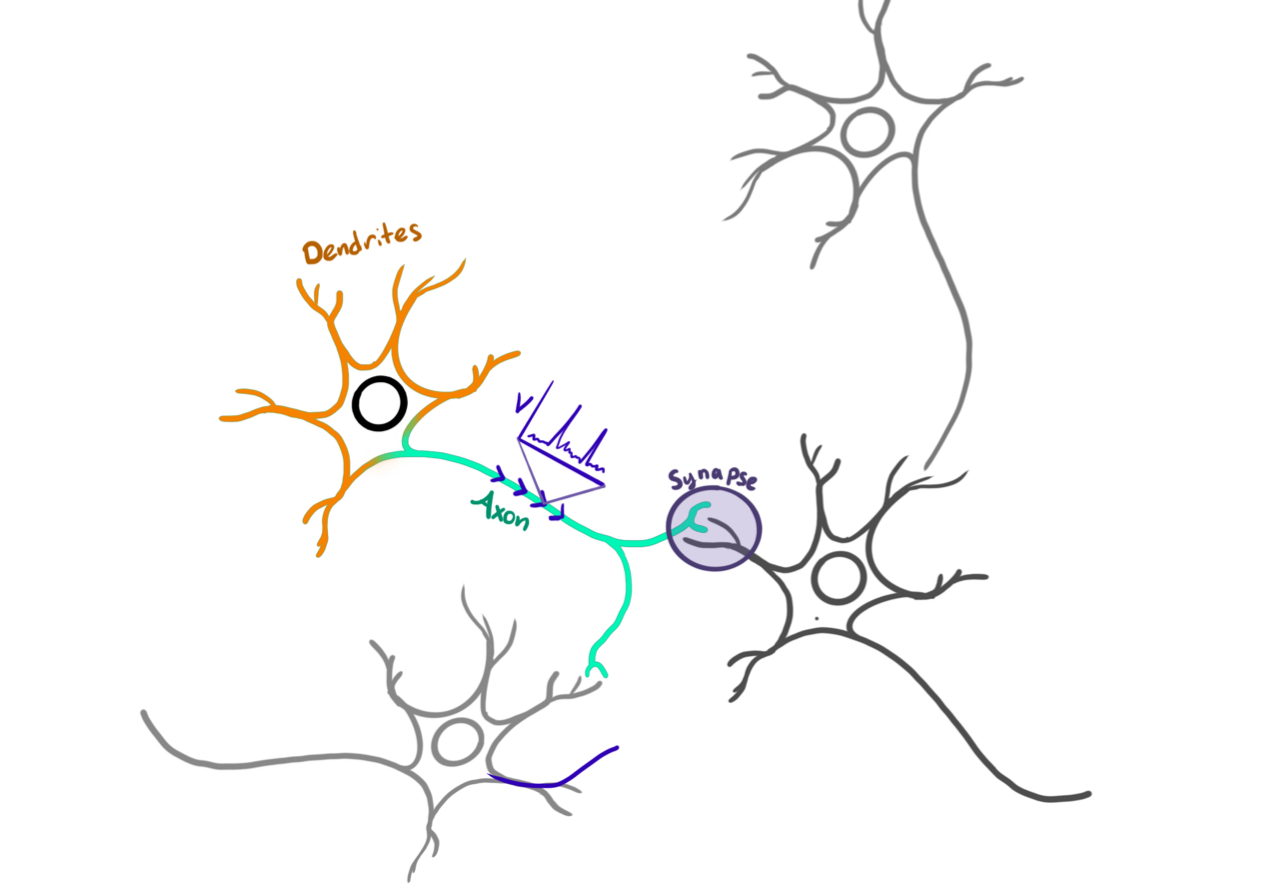
\includegraphics[width=\linewidth]{images/FILENAME}
	% Acknowledgements & References Example:
	\small{This work is supported by GRANT INFORMATION\\
		(1) AUTHORS (YEAR) \textit{JOURNAL}}
}

%%%%%%%%%%%%%%%%%%%
%%% Column 2
%%%%%%%%%%%%%%%%%%%
\headerbox{Spatial Error}{name = space, column = 2}{
	% Itemize Example:
	\begin{itemize}
		\setlength\itemsep{0pt}
		\small{
			\item \bf{Scientific Question}
		}
	\end{itemize}
	% Figure Example: 
	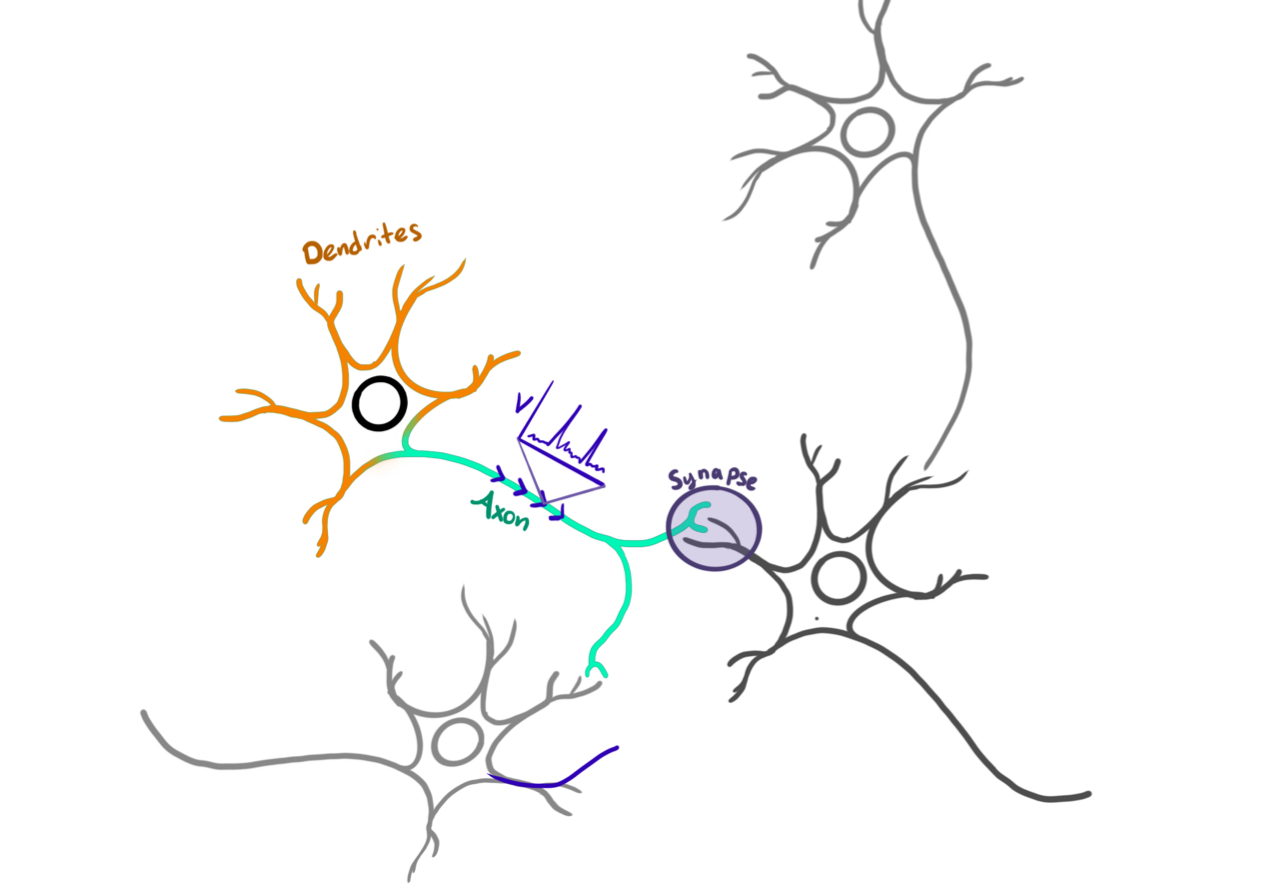
\includegraphics[width=\linewidth]{images/FILENAME}
	% Acknowledgements & References Example:
	\small{This work is supported by GRANT INFORMATION\\
		(1) AUTHORS (YEAR) \textit{JOURNAL}}
}

\headerbox{Convergence}{name = quad, column = 2, below=space}{
	% Itemize Example:
	\begin{itemize}
		\setlength\itemsep{0pt}
		\small{
			\item \bf{Scientific Question}
		}
	\end{itemize}
	% Figure Example: 
	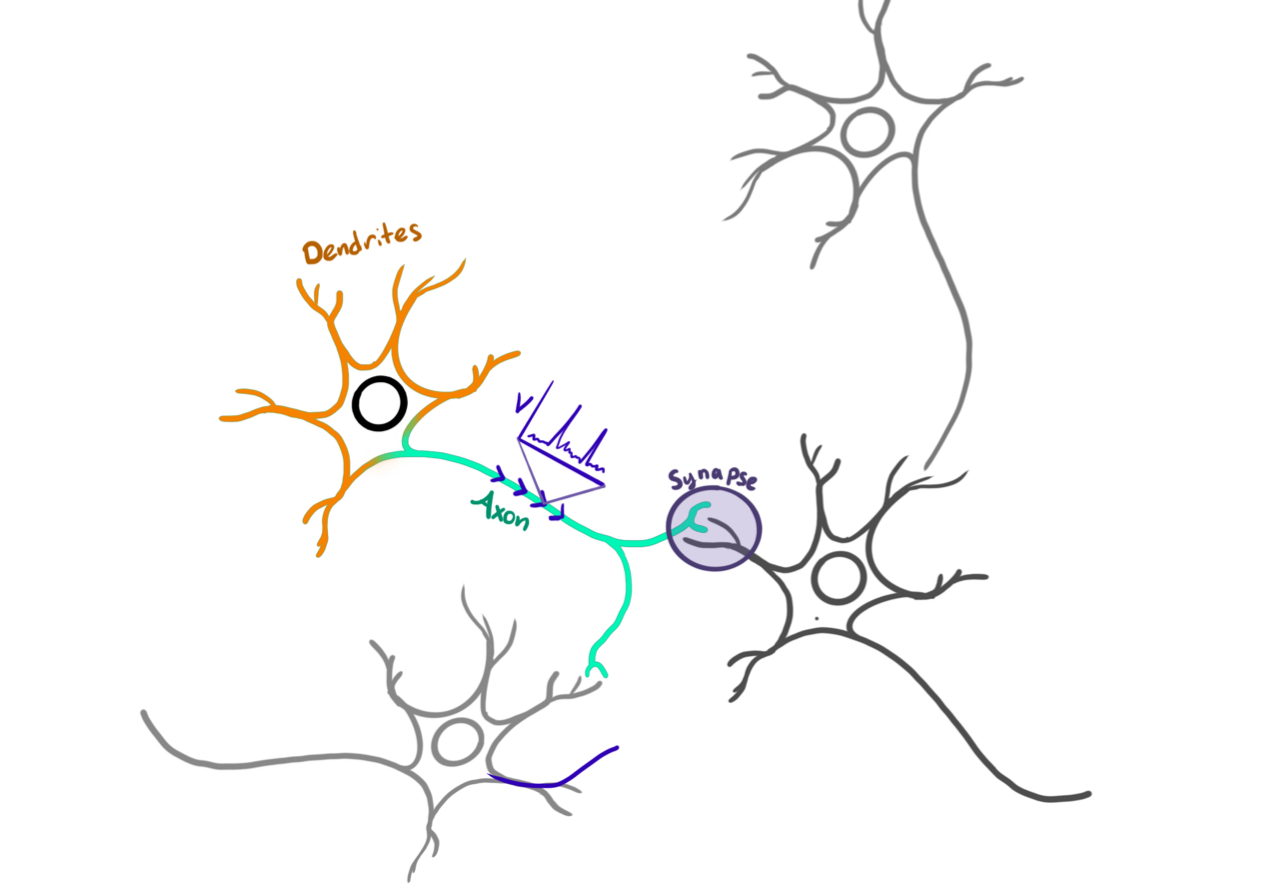
\includegraphics[width=\linewidth]{images/FILENAME}
	% Acknowledgements & References Example:
	\small{This work is supported by GRANT INFORMATION\\
		(1) AUTHORS (YEAR) \textit{JOURNAL}}
}

%%%%%%%%%%%%%%%%%%%
%%% Column 3
%%%%%%%%%%%%%%%%%%%
\headerbox{Neural Field IVP}{name = ivp, column = 3}{
	% Itemize Example:
	\begin{itemize}
		\setlength\itemsep{0pt}
		\small{
			\item \bf{Scientific Question}
		}
	\end{itemize}
	% Figure Example: 
	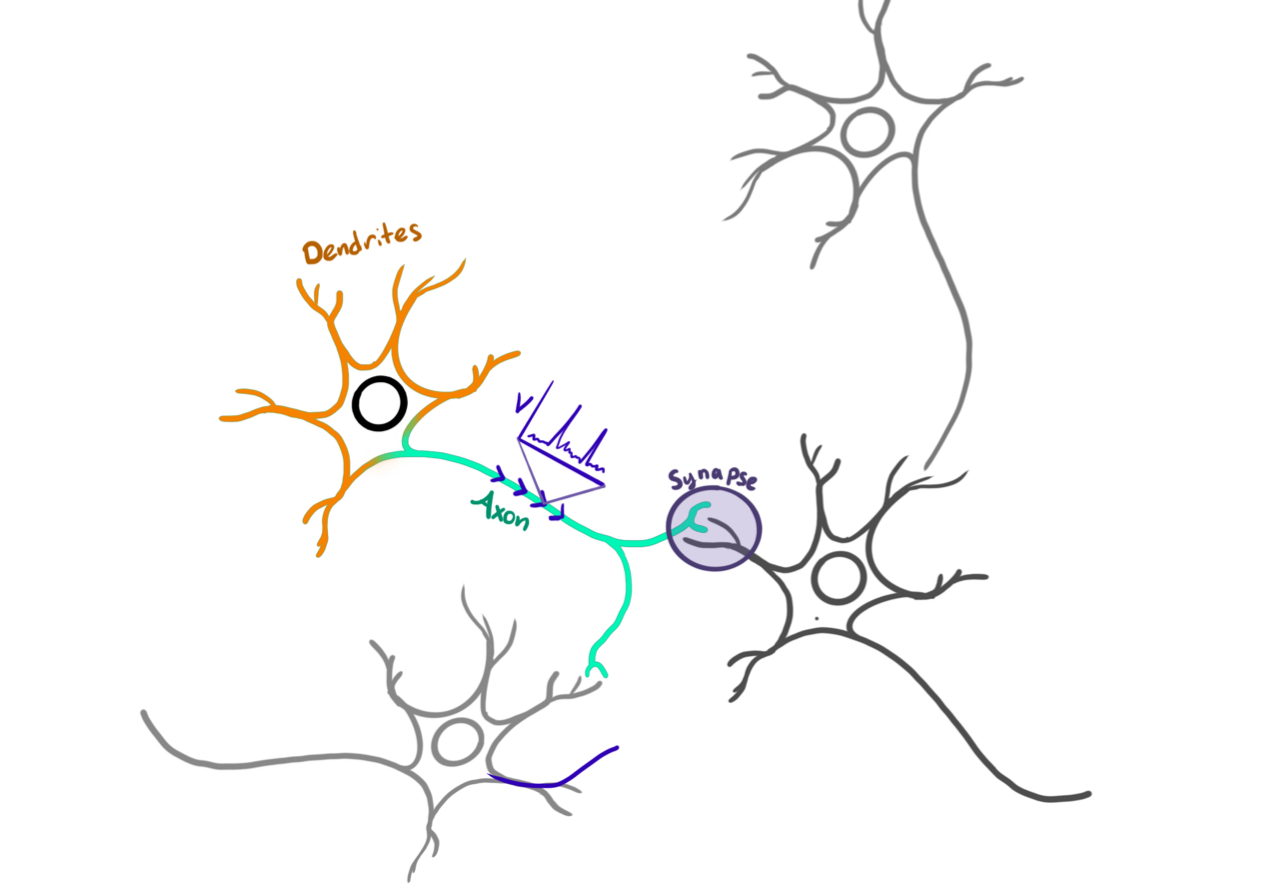
\includegraphics[width=\linewidth]{images/FILENAME}
	% Acknowledgements & References Example:
	\small{This work is supported by GRANT INFORMATION\\
		(1) AUTHORS (YEAR) \textit{JOURNAL}}
}

\headerbox{References and Funding}{name = ref, column = 3, below=ivp}{
	% Itemize Example:
	\begin{itemize}
		\setlength\itemsep{0pt}
		\small{
			\item Tsodyks, et al. (1998) Neural Computation
			\item Kilpatrick \& Bressloff (2010) Physica D 
			\item Kilpatrick \& Ermentrout (2012) Phys. Rev. E
This work was supported by NSF DMS-2207700.
		}
	\end{itemize}
	% Figure Example: 
	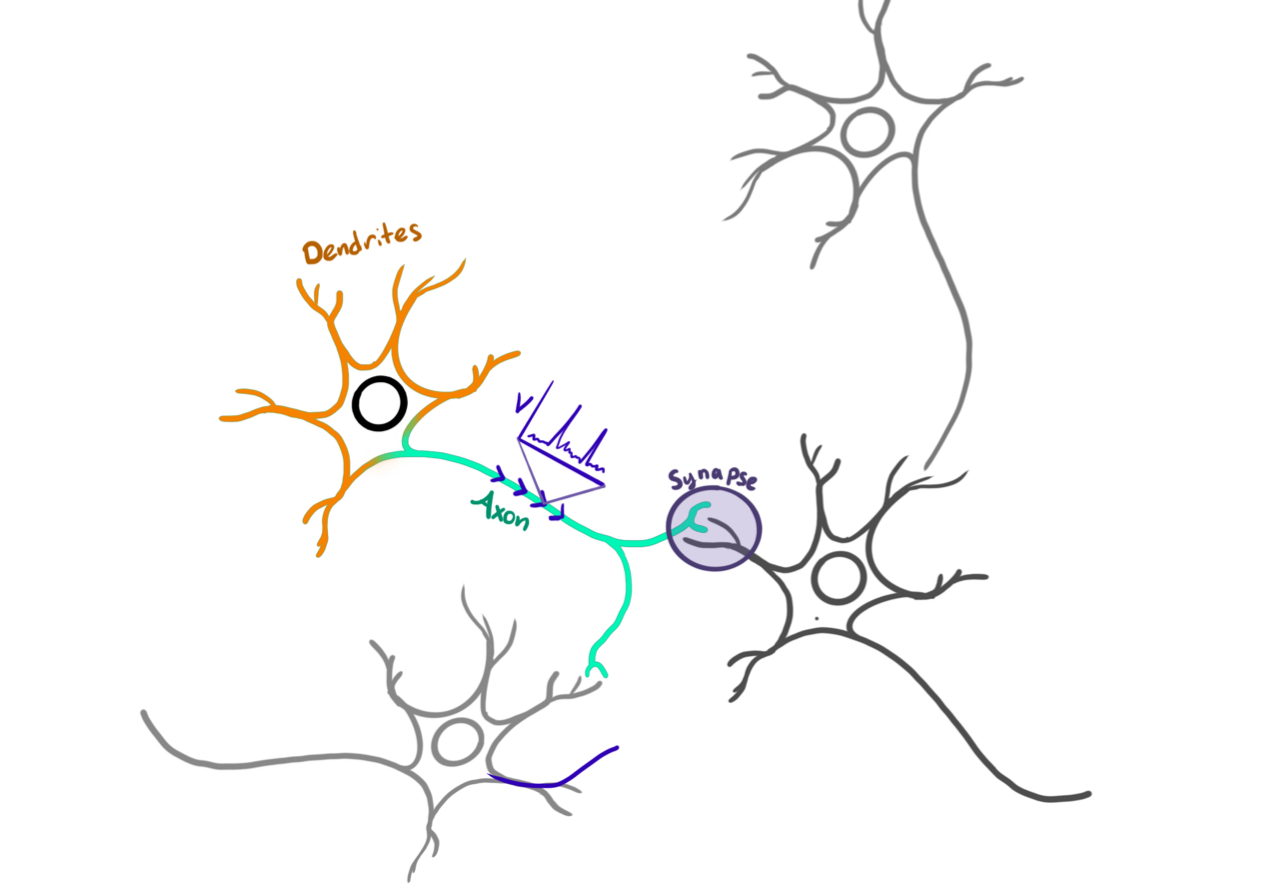
\includegraphics[width=\linewidth]{images/FILENAME}
	% Acknowledgements & References Example:
	\small{This work is supported by GRANT INFORMATION\\
		(1) AUTHORS (YEAR) \textit{JOURNAL}}
}

%%%%%%%%%%%%%%%%%%%%%%%%%%%%%%%%%%%%%%%%%%%%%
\end{poster}
\end{document}
